%%%%%%%%%%%%  Generated using docx2latex.com  %%%%%%%%%%%%%%

%%%%%%%%%%%%  v2.0.0-beta  %%%%%%%%%%%%%%

\documentclass[12pt,twoside]{article}
\usepackage{amsmath}
\usepackage{latexsym}
\usepackage{amsfonts}
\usepackage[normalem]{ulem}
\usepackage{array}
\usepackage{amssymb}
\usepackage{graphicx}
\usepackage[backend=biber,
style=numeric,
sorting=none,
isbn=false,
doi=false,
url=false,
]{biblatex}\addbibresource{bibliography.bib}

\usepackage{subfig}
\usepackage{wrapfig}
\usepackage{wasysym}
\usepackage{enumitem}
\usepackage{adjustbox}
\usepackage{ragged2e}
\usepackage[svgnames,table]{xcolor}
\usepackage{tikz}
\usepackage{longtable}
\usepackage{changepage}
\usepackage{setspace}
\usepackage{hhline}
\usepackage{multicol}
\usepackage{tabto}
\usepackage{float}
\usepackage{multirow}
\usepackage{makecell}
\usepackage{fancyhdr}
\usepackage[toc,page]{appendix}
\usepackage[hidelinks]{hyperref}
\usetikzlibrary{shapes.symbols,shapes.geometric,shadows,arrows.meta}
\tikzset{>={Latex[width=1.5mm,length=2mm]}}
\usepackage{flowchart}\usepackage[paperheight=11.0in,paperwidth=8.5in,left=0.67in,right=0.67in,top=1.04in,bottom=0.19in,headheight=1in]{geometry}
\usepackage[utf8]{inputenc}
\usepackage[T1]{fontenc}
\TabPositions{0.5in,1.0in,1.5in,2.0in,2.5in,3.0in,3.5in,4.0in,4.5in,5.0in,5.5in,6.0in,6.5in,7.0in,}

\urlstyle{same}


 %%%%%%%%%%%%  Set Depths for Sections  %%%%%%%%%%%%%%

% 1) Section
% 1.1) SubSection
% 1.1.1) SubSubSection
% 1.1.1.1) Paragraph
% 1.1.1.1.1) Subparagraph


\setcounter{tocdepth}{5}
\setcounter{secnumdepth}{5}


 %%%%%%%%%%%%  Set Depths for Nested Lists created by \begin{enumerate}  %%%%%%%%%%%%%%


\setlistdepth{9}
\renewlist{enumerate}{enumerate}{9}
		\setlist[enumerate,1]{label=\arabic*)}
		\setlist[enumerate,2]{label=\alph*)}
		\setlist[enumerate,3]{label=(\roman*)}
		\setlist[enumerate,4]{label=(\arabic*)}
		\setlist[enumerate,5]{label=(\Alph*)}
		\setlist[enumerate,6]{label=(\Roman*)}
		\setlist[enumerate,7]{label=\arabic*}
		\setlist[enumerate,8]{label=\alph*}
		\setlist[enumerate,9]{label=\roman*}

\renewlist{itemize}{itemize}{9}
		\setlist[itemize]{label=$\cdot$}
		\setlist[itemize,1]{label=\textbullet}
		\setlist[itemize,2]{label=$\circ$}
		\setlist[itemize,3]{label=$\ast$}
		\setlist[itemize,4]{label=$\dagger$}
		\setlist[itemize,5]{label=$\triangleright$}
		\setlist[itemize,6]{label=$\bigstar$}
		\setlist[itemize,7]{label=$\blacklozenge$}
		\setlist[itemize,8]{label=$\prime$}



 %%%%%%%%%%%%  Header here  %%%%%%%%%%%%%%


\pagestyle{fancy}
\fancyhf{}
\fancyfoot[LE,RO]{\thepage}
\renewcommand{\headrulewidth}{0pt}
\setlength{\topsep}{0pt}\setlength{\parindent}{0pt}
\renewcommand{\arraystretch}{1.3}


%%%%%%%%%%%%%%%%%%%% Document code starts here %%%%%%%%%%%%%%%%%%%%



\begin{document}

\vspace{\baselineskip}

\vspace{\baselineskip}
\begin{adjustwidth}{0.6in}{0.0in}
\par

\end{adjustwidth}


\vspace{\baselineskip}

\vspace{\baselineskip}
\begin{itemize}
	\item Introduction\par


\vspace{\baselineskip}
{\fontsize{10pt}{12.0pt}\selectfont The main objective of this final lecture is to briefly introduce the concept of decision making under uncer- tainty, which essentially deals with the higher level of\ the decision making module whereby one is trying  to reason about what the other agents in the environment are doing. A useful way of reasoning about the uncertainty of the environment is model the environment as probabilistic. This results in the development of control policies that optimize the dynamical system that evolves through time probabilistically.\par}\par


\vspace{\baselineskip}

\vspace{\baselineskip}
	\item Basic Decision Making Problem\par

\begin{itemize}
	\item {\fontsize{10pt}{12.0pt}\selectfont System: \textit{x\textsubscript{k}}\textsubscript{+1} = \textit{f\textsubscript{k}}(\textit{x\textsubscript{k}}, \textit{u\textsubscript{k}}, \textit{w\textsubscript{k}}), \textit{k }= 0, . . . , \textit{N}\par}\par

\begin{itemize}
	\item {\fontsize{10pt}{12.0pt}\selectfont Very similar to the dynamics studied in the context of filtering.\par}\par


\end{itemize}
	\item {\fontsize{10pt}{12.0pt}\selectfont Control constraints: \textit{u\textsubscript{k} }$ \in $  \textit{U}(\textit{x\textsubscript{k}})\par}\par

	\item {\fontsize{10pt}{12.0pt}\selectfont Probability distribution:  \textit{P\textsubscript{k}}($ \vert $ ˙\textit{x\textsubscript{k}}, \textit{u\textsubscript{k}}) of \textit{w\textsubscript{k}}\par}\par

\begin{itemize}
	\item {\fontsize{10pt}{12.0pt}\selectfont The disturbance the affects the dynamics has a probability distribution that only depends on the current state \textit{x\textsubscript{k} }and current control \textit{u\textsubscript{k} }(Markov assumption).\par}\par


\end{itemize}
	\item {\fontsize{10pt}{12.0pt}\selectfont Policies: \textit{$ \pi $  }= $ \{ $ \textit{$ \mu $ }\textsubscript{0}, . . . , \textit{$ \mu $ \textsubscript{N}}\textsubscript{$-$ 1}$ \} $ , where \textit{u\textsubscript{k} }= \textit{$ \mu $ k }(\textit{x\textsubscript{k}})\par}\par

\begin{itemize}
	\item {\fontsize{10pt}{12.0pt}\selectfont Interested in optimizing closed-loop policy in stochastic context for robustness.\par}\par


\end{itemize}
	\item {\fontsize{10pt}{12.0pt}\selectfont Expected Cost:\par}\par


\vspace{\baselineskip}

\end{itemize}
\end{itemize}\begin{FlushRight}
{\fontsize{10pt}{12.0pt}\selectfont \textit{J\textsubscript{$ \pi $ } }(\par}
\end{FlushRight}\par

\begin{FlushLeft}
\\
{\fontsize{10pt}{12.0pt}\selectfont \textit{x}\textsubscript{0}) =\par}
\end{FlushLeft}\par

\begin{FlushLeft}
\\
{\fontsize{10pt}{12.0pt}\selectfont \textit{E},\textit{g\textsubscript{N} }(\textit{x}\par}
\end{FlushLeft}\par

\begin{FlushLeft}
\\
{\fontsize{7pt}{8.4pt}\selectfont \textit{N }{\fontsize{10pt}{12.0pt}\selectfont ) +\par}\par}
\end{FlushLeft}\par

\begin{FlushLeft}
\\
{\fontsize{7pt}{8.4pt}\selectfont \textit{N}$-$ 1\par}
\end{FlushLeft}\par

\begin{FlushRight}
{\fontsize{7pt}{8.4pt}\selectfont \textit{k }{\fontsize{10pt}{12.0pt}\selectfont (\par}\par}
\end{FlushRight}\par

\begin{FlushLeft}
{\fontsize{7pt}{8.4pt}\selectfont \textit{k}=1\par}
\end{FlushLeft}\par

\begin{FlushLeft}
\\
{\fontsize{10pt}{12.0pt}\selectfont \textit{x\textsubscript{k}}, \textit{$ \mu $ k }(\par}
\end{FlushLeft}\par

\begin{FlushLeft}
\\
{\fontsize{10pt}{12.0pt}\selectfont \textit{x\textsubscript{k}}), \textit{w\textsubscript{k}}),\par}
\end{FlushLeft}\par


\vspace{\baselineskip}
{\fontsize{10pt}{12.0pt}\selectfont \textbf{– \textit{g\textsubscript{N is the terminal cost and gk is the stage-wise cost (note the additive structure of the cost function).}}}\par}\par


\vspace{\baselineskip}
\begin{itemize}
	\item \begin{itemize}
	\item \begin{itemize}
	\item {\fontsize{10pt}{12.0pt}\selectfont Decision making problem:\tab \textit{J}{\fontsize{7pt}{8.4pt}\selectfont $\ast$ \par}\par}\par

\\

\vspace{\baselineskip}{\fontsize{10pt}{12.0pt}\selectfont (\textit{x\textsubscript{0) =}}\par}\par

\\

\vspace{\baselineskip}\begin{FlushLeft}
{\fontsize{10pt}{12.0pt}\selectfont min \textit{J\textsubscript{$ \pi $ } }(\par}
\end{FlushLeft}\par

\begin{FlushLeft}
{\fontsize{7pt}{8.4pt}\selectfont \textit{$ \pi $ }\par}
\end{FlushLeft}\par

\\

\vspace{\baselineskip}\begin{FlushLeft}
{\fontsize{10pt}{12.0pt}\selectfont \textit{x}\textsubscript{0})\par}
\end{FlushLeft}\par


\vspace{\baselineskip}

\end{itemize}
\end{itemize}
\end{itemize}
\vspace{\baselineskip}
{\fontsize{10pt}{12.0pt}\selectfont Key points:\par}\par


\vspace{\baselineskip}
\begin{itemize}
	\item \begin{itemize}
	\item \begin{itemize}
	\item {\fontsize{10pt}{12.0pt}\selectfont Discrete-time model\par}\par

\begin{itemize}
	\item {\fontsize{10pt}{12.0pt}\selectfont Could consider continuous-time model, but in most applications the discrete-time is most nat- ural.\par}\par


\vspace{\baselineskip}
{\fontsize{10pt}{12.0pt}\selectfont 18-1\par}\par


\vspace{\baselineskip}

\end{itemize}
\end{itemize}
\end{itemize}
\end{itemize}
\vspace{\baselineskip}
\begin{itemize}
	\item {\fontsize{10pt}{12.0pt}\selectfont Markovian model\par}\par

	\item {\fontsize{10pt}{12.0pt}\selectfont Objective: find optimal closed-loop policy\par}\par

	\item {\fontsize{10pt}{12.0pt}\selectfont Additive cost (central assumption to prove the principle of optimality)\par}\par

	\item {\fontsize{10pt}{12.0pt}\selectfont Risk-neutral formulation\par}\par


\vspace{\baselineskip}
	\item Principle of Optimality
\end{itemize}\par


\vspace{\baselineskip}
\begin{adjustwidth}{0.08in}{0.0in}
{\fontsize{10pt}{12.0pt}\selectfont The principle of optimality is a key concept to make stochastic optimal control problem tractable from a computational standpoint.\par}\par

\end{adjustwidth}

\begin{adjustwidth}{0.08in}{0.54in}
{\fontsize{10pt}{12.0pt}\selectfont Consider the simplest case (deterministic, i.e. no stochasticity), and suppose the optimal path for a multi- stage decision-making problem is shown by the figure below\par}\par

\end{adjustwidth}


\vspace{\baselineskip}

\vspace{\baselineskip}


%%%%%%%%%%%%%%%%%%%% Figure/Image No: 1 starts here %%%%%%%%%%%%%%%%%%%%

\begin{figure}[H]
\advance\leftskip 2.75in		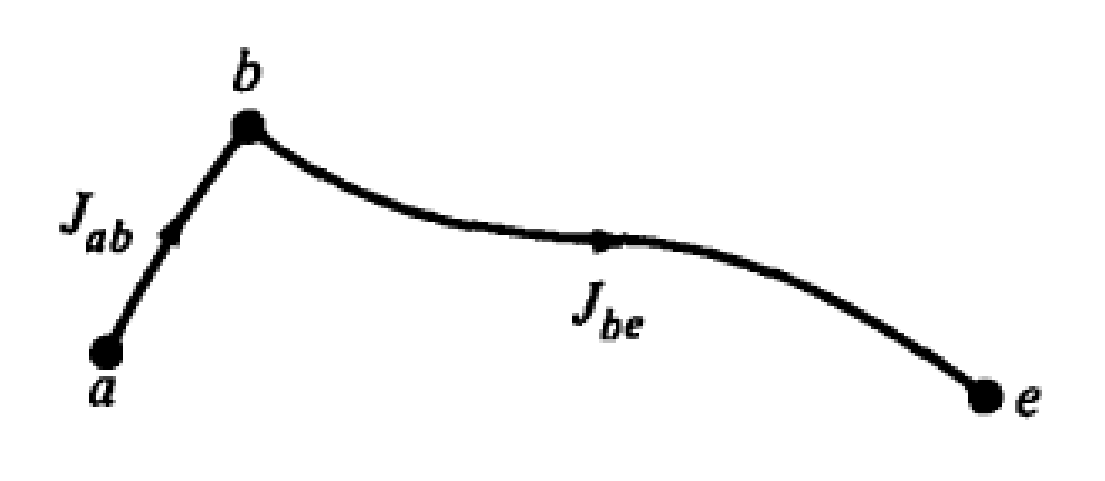
\includegraphics[width=2.46in,height=0.93in]{./media/image1.jpeg}
\end{figure}


%%%%%%%%%%%%%%%%%%%% Figure/Image No: 1 Ends here %%%%%%%%%%%%%%%%%%%%

{\fontsize{10pt}{12.0pt}\selectfont \par}\par


\vspace{\baselineskip}
\begin{adjustwidth}{0.08in}{0.54in}
where the first decision yields segment a-b with cost \textit{J\textsubscript{ab}}, and remaining decisions yield segments b-e with cost \textit{J\textsubscript{be}}. The total optimal cost is then \textit{J\textsubscript{a}}$\ast$ \textit{e }= \textit{J\textsubscript{ab} }+ \textit{J\textsubscript{be}}.\par

\end{adjustwidth}

\begin{adjustwidth}{0.08in}{0.64in}
{\fontsize{10pt}{12.0pt}\selectfont The\ big\ claim of the principle of optimality is as follows:  if a-b-e is an optimal path from a to e, then b-e  is an optimal path from b to e.\par}\par

\end{adjustwidth}

\begin{adjustwidth}{0.08in}{0.0in}
{\fontsize{10pt}{12.0pt}\selectfont Proof by contradiction: Suppose b-c-e is the optimal path from b to e. Then\par}\par

\end{adjustwidth}


\vspace{\baselineskip}

\vspace{\baselineskip}
\begin{multicols}{2}

\vspace{\baselineskip}
{\fontsize{10pt}{12.0pt}\selectfont and\par}\par

\begin{Center}
\\
{\fontsize{10pt}{12.0pt}\selectfont \textit{J}{\fontsize{7pt}{8.4pt}\selectfont \textit{bce\  }{\fontsize{10pt}{12.0pt}\selectfont \textit{< J}{\fontsize{7pt}{8.4pt}\selectfont \textit{be}\par}\par}\par}\par}
\end{Center}\par


\vspace{\baselineskip}
\begin{Center}
{\fontsize{10pt}{12.0pt}\selectfont \textit{J}{\fontsize{7pt}{8.4pt}\selectfont \textit{ab }{\fontsize{10pt}{12.0pt}\selectfont + \textit{J}{\fontsize{7pt}{8.4pt}\selectfont \textit{bce }{\fontsize{10pt}{12.0pt}\selectfont \textit{< J}{\fontsize{7pt}{8.4pt}\selectfont \textit{ab }{\fontsize{10pt}{12.0pt}\selectfont + \textit{J}{\fontsize{7pt}{8.4pt}\selectfont \textit{be }{\fontsize{10pt}{12.0pt}\selectfont = \textit{J}{\fontsize{7pt}{8.4pt}\selectfont \textit{a}$\ast$ \textit{e}\par}\par}\par}\par}\par}\par}\par}\par}\par}\par}
\end{Center}\par


\vspace{\baselineskip}

\end{multicols}

\vspace{\baselineskip}

\vspace{\baselineskip}

\vspace{\baselineskip}


%%%%%%%%%%%%%%%%%%%% Figure/Image No: 2 starts here %%%%%%%%%%%%%%%%%%%%

\begin{figure}[H]
	\begin{Center}
		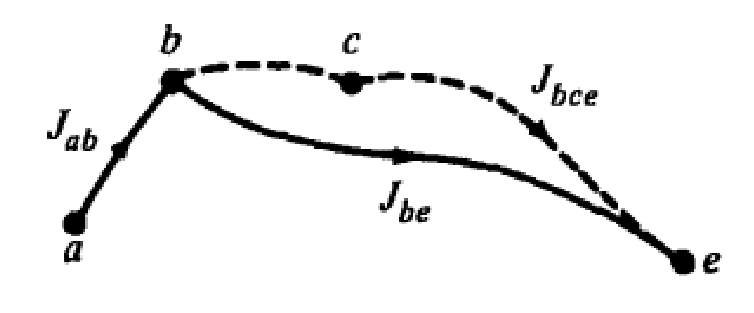
\includegraphics[width=2.46in,height=0.92in]{./media/image2.jpeg}
	\end{Center}
\end{figure}


%%%%%%%%%%%%%%%%%%%% Figure/Image No: 2 Ends here %%%%%%%%%%%%%%%%%%%%

{\fontsize{10pt}{12.0pt}\selectfont \par}\par


\vspace{\baselineskip}

\vspace{\baselineskip}
\begin{adjustwidth}{0.08in}{0.58in}
This is a contradiction because \textit{J\textsubscript{a}}$\ast$ \textit{e }is already defined as the optimal path from a to e. If \textit{J\textsubscript{bce} }was optimal path from b to e instead of \textit{J\textsubscript{be}}, then that would imply that \textit{J\textsubscript{a}}$\ast$ \textit{e }is not optimal. Therefore, \textit{J\textsubscript{be} }must be the optimal path from b to e.\par

\end{adjustwidth}


\vspace{\baselineskip}

\vspace{\baselineskip}
\begin{adjustwidth}{0.58in}{0.08in}
{\fontsize{10pt}{12.0pt}\selectfont \textbf{Remark: While\ the principle of optimality holds for tails of optimal policies, the same is not true for  heads of optimal policies. Consider the simple game where there are two strategies \textit{$ \pi $ \textsubscript{1, $ \pi $ 2. The costs as a function of time for these strategies are}}}\par}\par

\end{adjustwidth}

\begin{adjustwidth}{3.48in}{2.99in}
\begin{Center}
{\fontsize{10pt}{12.0pt}\selectfont \textit{r}\textsubscript{1}(\textit{t}) = 10\textit{t r}\textsubscript{2}(\textit{t}) = \textit{e}0.1\textit{t}\par}
\end{Center}\par

\end{adjustwidth}

\begin{adjustwidth}{0.58in}{0.0in}
{\fontsize{10pt}{12.0pt}\selectfont and the goal of the game is to accumulate as much reward as possible for the duration of the game.\par}\par

\end{adjustwidth}

\begin{adjustwidth}{1.18in}{0.0in}
\begin{Center}
{\fontsize{7pt}{8.4pt}\selectfont \textit{T}\par}
\end{Center}\par

\end{adjustwidth}

\begin{adjustwidth}{0.85in}{0.35in}
\begin{Center}
{\fontsize{10pt}{12.0pt}\selectfont \textit{$ \pi $ }{\fontsize{7pt}{8.4pt}\selectfont \textit{T}$\ast$   {\fontsize{10pt}{12.0pt}\selectfont = arg  min\   {\fontsize{14pt}{16.8pt}\selectfont $ \sum $  {\fontsize{10pt}{12.0pt}\selectfont \textit{r\textsubscript{i}}(\textit{t})\par}\par}\par}\par}\par}
\end{Center}\par

\end{adjustwidth}

\begin{adjustwidth}{3.71in}{0.0in}
\begin{FlushLeft}
{\fontsize{7pt}{8.4pt}\selectfont \textit{i}$ \in $ $ \{ $ 1,2$ \} $  \textit{t}=1\par}
\end{FlushLeft}\par

\end{adjustwidth}

\begin{adjustwidth}{0.58in}{0.54in}
It is easy to check that for \textit{T }= 5, the optimal policy is \textit{$ \pi $ }\textsubscript{2}, but if \textit{T }= 1000, the optimal policy is \textit{$ \pi $ }\textsubscript{1}. However, the behavior of \textit{$ \pi $ }1$\ast$ 000  during the first 5 timesteps is not the same as the behavior of \textit{$ \pi $ }5$\ast$ .\par

\end{adjustwidth}


\vspace{\baselineskip}
\begin{itemize}
	\item Definition (for discrete-time systems)\par


\vspace{\baselineskip}
Let\  \textbf{\textit{f }}{\fontsize{7pt}{8.4pt}\selectfont $\ast$  \par}:=\ \  \textbf{\textit{f}}{\fontsize{7pt}{8.4pt}\selectfont 0$\ast$ \par}, \textbf{\textit{f}}{\fontsize{7pt}{8.4pt}\selectfont 1$\ast$ \par}, . . . , \textbf{\textit{f}}{\fontsize{7pt}{8.4pt}\selectfont \textit{N}$\ast$ \ \  1\ \ \ \  \par}be an optimal policy. Assume state \textbf{\textit{x}}\textit{\textsubscript{k} }is reachable. Consider the subproblem whereby we are at \textbf{\textit{x}}\textit{\textsubscript{k} }at time \textit{k }and we wish to minimize the cost-to-go from time \textit{k }to time \textit{N}. Then, the truncated policy $ \{ $  \textbf{\textit{f}}\textit{k}$\ast$ , \textbf{\textit{f}}\textit{k}$\ast$ +1, . . . , \textbf{\textit{f}}\textit{N}$\ast$  $-$ 1$ \} $  is optimal for the subproblem.\par

Considering this definition, \textit{tail }policies are optimal for \textit{tail }subproblems. Also, mind that the time- dependence is implicit in the notation: \textbf{\textit{f}}{\fontsize{7pt}{8.4pt}\selectfont \textit{k}$\ast$  \par}(\textbf{\textit{x}}\textit{\textsubscript{k}}) = \textbf{\textit{f }}$\ast$  (\textbf{\textit{x}}\textit{\textsubscript{k}}, \textit{k}).\par


\vspace{\baselineskip}
	\item Applying the principle of optimality\par


\vspace{\baselineskip}
{\fontsize{10pt}{12.0pt}\selectfont Consider the problem shown in the figure below.\par}\par


\vspace{\baselineskip}


%%%%%%%%%%%%%%%%%%%% Figure/Image No: 3 starts here %%%%%%%%%%%%%%%%%%%%

\begin{figure}[H]
\advance\leftskip 3.18in		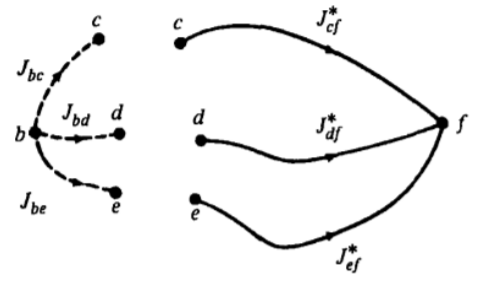
\includegraphics[width=2.61in,height=1.54in]{./media/image3.jpeg}
\end{figure}


%%%%%%%%%%%%%%%%%%%% Figure/Image No: 3 Ends here %%%%%%%%%%%%%%%%%%%%

{\fontsize{10pt}{12.0pt}\selectfont \par}\par


\vspace{\baselineskip}
{\fontsize{10pt}{12.0pt}\selectfont According to the principle of optimality,\  if\  \textit{b\  c is\ the initial segment of the optimal path from  b to\  f ,\ \  then c f is the terminal segment of this path. Hence, the optimal trajectory is found by comparing the following:}\par}\par

\begin{justify}
{\fontsize{10pt}{12.0pt}\selectfont \textit{C}{\fontsize{7pt}{8.4pt}\selectfont \textit{bc f }{\fontsize{10pt}{12.0pt}\selectfont = \textit{J}{\fontsize{7pt}{8.4pt}\selectfont \textit{bc }{\fontsize{10pt}{12.0pt}\selectfont + \textit{J}{\fontsize{7pt}{8.4pt}\selectfont \textit{c}$\ast$ \textit{f }{\fontsize{10pt}{12.0pt}\selectfont \textit{C}{\fontsize{7pt}{8.4pt}\selectfont \textit{bd f\  }{\fontsize{10pt}{12.0pt}\selectfont = \textit{J}{\fontsize{7pt}{8.4pt}\selectfont \textit{bd }{\fontsize{10pt}{12.0pt}\selectfont + \textit{J}{\fontsize{7pt}{8.4pt}\selectfont \textit{d}$\ast$ \textit{f }{\fontsize{10pt}{12.0pt}\selectfont \textit{C}{\fontsize{7pt}{8.4pt}\selectfont \textit{be f }{\fontsize{10pt}{12.0pt}\selectfont = \textit{J}{\fontsize{7pt}{8.4pt}\selectfont \textit{be }{\fontsize{10pt}{12.0pt}\selectfont + \textit{J}{\fontsize{7pt}{8.4pt}\selectfont \textit{e}$\ast$ \textit{f}\par}\par}\par}\par}\par}\par}\par}\par}\par}\par}\par}\par}\par}\par}\par}\par}\par}\par}
\end{justify}\par

{\fontsize{10pt}{12.0pt}\selectfont The comparison of these three trajectories is shown in the figure below.\par}\par


\vspace{\baselineskip}

\end{itemize}
\vspace{\baselineskip}

\vspace{\baselineskip}

\vspace{\baselineskip}


%%%%%%%%%%%%%%%%%%%% Figure/Image No: 4 starts here %%%%%%%%%%%%%%%%%%%%

\begin{figure}[H]
	\begin{Center}
		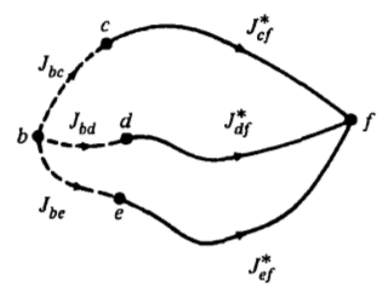
\includegraphics[width=2.59in,height=1.95in]{./media/image4.jpeg}
	\end{Center}
\end{figure}


%%%%%%%%%%%%%%%%%%%% Figure/Image No: 4 Ends here %%%%%%%%%%%%%%%%%%%%

{\fontsize{10pt}{12.0pt}\selectfont \par}\par


\vspace{\baselineskip}

\vspace{\baselineskip}
{\fontsize{10pt}{12.0pt}\selectfont When applying the principle of optimality, one only needs to compare the concatenations of immediate decisions and optimal decisions. This provides a significant decrease in the computation required to solve the problem, and also the amount of possible solutions.\par}\par

{\fontsize{10pt}{12.0pt}\selectfont In practice, the principle of optimality is applied \textit{backward in time. As Soren Kierkegaard said, $``$Life can only be understood backwards; but it must be lived forwards.$"$ }\par}\par


\vspace{\baselineskip}

\vspace{\baselineskip}
\begin{itemize}
	\item \begin{itemize}
	\item \begin{itemize}
	\item Example problem
\end{itemize}
\end{itemize}
\end{itemize}\par


\vspace{\baselineskip}
\begin{adjustwidth}{0.08in}{0.58in}
{\fontsize{10pt}{12.0pt}\selectfont As an example of solving a problem with the principle of optimality,\  consider the figure below.\  The\ goal\   is to start from node \textit{a and end at node h while incurring the minimum cost along the path. Consider the following movement map: [North: UP], [South: DOWN], [East: RIGHT], [West: LEFT].}\par}\par

\end{adjustwidth}


\vspace{\baselineskip}

\vspace{\baselineskip}


%%%%%%%%%%%%%%%%%%%% Figure/Image No: 5 starts here %%%%%%%%%%%%%%%%%%%%

\begin{figure}[H]
\advance\leftskip 1.22in		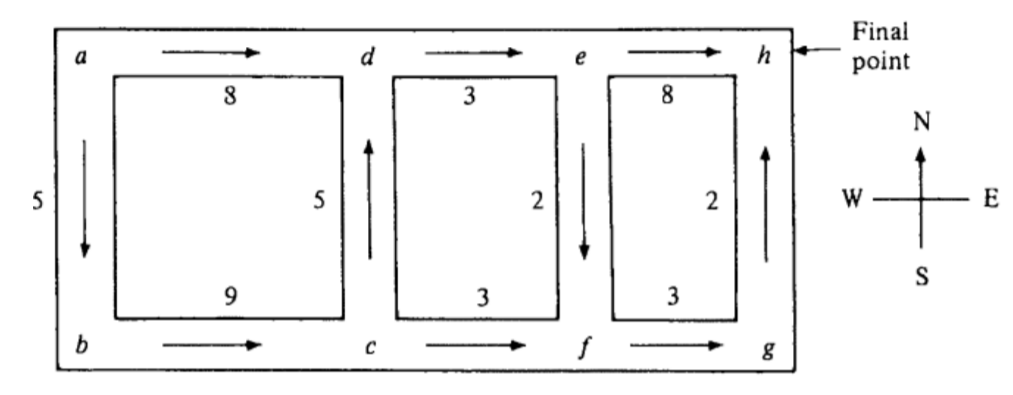
\includegraphics[width=5.65in,height=2.08in]{./media/image5.jpeg}
\end{figure}


%%%%%%%%%%%%%%%%%%%% Figure/Image No: 5 Ends here %%%%%%%%%%%%%%%%%%%%

{\fontsize{10pt}{12.0pt}\selectfont \par}\par


\vspace{\baselineskip}

\vspace{\baselineskip}
\begin{adjustwidth}{0.08in}{0.58in}
As mentioned earlier, in practice, the principle of optimality is applied backward in time. First, consider the cost-to-go from starting at node \textit{h}: \textit{J}(\textit{h}) = 0.\ Then, consider the cost-to-go and optimal action for  node \textit{g}: \textit{J}(\textit{g}) = 2 + \textit{J}(\textit{h}) = 2 + 0 = 2, \textit{u}{\fontsize{7pt}{8.4pt}\selectfont $\ast$  \par}(\textit{g}) = \textit{UP}. Continuing for the rest of the problem, we have the following:\par

\end{adjustwidth}


\vspace{\baselineskip}

\vspace{\baselineskip}

\vspace{\baselineskip}

\vspace{\baselineskip}
\begin{adjustwidth}{0.51in}{1.09in}
{\fontsize{10pt}{12.0pt}\selectfont \textit{J( f ) = 3 + J(g) = 3 + 2 = 5}\par}\par

\end{adjustwidth}

\begin{adjustwidth}{2.35in}{0.0in}
\begin{FlushLeft}
{\fontsize{10pt}{12.0pt}\selectfont \textit{u}{\fontsize{7pt}{8.4pt}\selectfont $\ast$  {\fontsize{10pt}{12.0pt}\selectfont ( \textit{f }) = \textit{RIGHT}\par}\par}\par}
\end{FlushLeft}\par

\end{adjustwidth}


\vspace{\baselineskip}
\begin{adjustwidth}{0.51in}{1.09in}
{\fontsize{10pt}{12.0pt}\selectfont \textit{J( f ) = 3 + J(g) = 3 + 2 = 5}\par}\par

\end{adjustwidth}

\begin{adjustwidth}{2.35in}{0.0in}
\begin{FlushLeft}
{\fontsize{10pt}{12.0pt}\selectfont \textit{u}{\fontsize{7pt}{8.4pt}\selectfont $\ast$  {\fontsize{10pt}{12.0pt}\selectfont ( \textit{f }) = \textit{RIGHT}\par}\par}\par}
\end{FlushLeft}\par

\end{adjustwidth}


\vspace{\baselineskip}
\begin{adjustwidth}{2.46in}{0.0in}
{\fontsize{10pt}{12.0pt}\selectfont \textit{J(e) = min(8 + J(h) = 8, 2 + J( f ) = 7) = 7}\par}\par

\end{adjustwidth}

\begin{adjustwidth}{2.37in}{0.0in}
\begin{FlushLeft}
{\fontsize{10pt}{12.0pt}\selectfont \textit{u}{\fontsize{7pt}{8.4pt}\selectfont $\ast$  {\fontsize{10pt}{12.0pt}\selectfont (\textit{e}) = \textit{DOW N}\par}\par}\par}
\end{FlushLeft}\par

\end{adjustwidth}


\vspace{\baselineskip}
\begin{adjustwidth}{0.07in}{1.09in}
{\fontsize{10pt}{12.0pt}\selectfont \textit{J(d) = 3 + J(e) = 10}\par}\par

\end{adjustwidth}

\begin{adjustwidth}{2.36in}{0.0in}
\begin{FlushLeft}
{\fontsize{10pt}{12.0pt}\selectfont \textit{u}{\fontsize{7pt}{8.4pt}\selectfont $\ast$  {\fontsize{10pt}{12.0pt}\selectfont (\textit{d}) = \textit{RIGHT}\par}\par}\par}
\end{FlushLeft}\par

\end{adjustwidth}


\vspace{\baselineskip}
\begin{adjustwidth}{2.46in}{0.0in}
{\fontsize{10pt}{12.0pt}\selectfont \textit{J(c) = min(5 + J(d) = 15, 3 + J( f ) = 8) = 8}\par}\par

\end{adjustwidth}

\begin{adjustwidth}{2.37in}{0.0in}
\begin{FlushLeft}
{\fontsize{10pt}{12.0pt}\selectfont \textit{u}{\fontsize{7pt}{8.4pt}\selectfont $\ast$  {\fontsize{10pt}{12.0pt}\selectfont (\textit{c}) = \textit{RIGHT}\par}\par}\par}
\end{FlushLeft}\par

\end{adjustwidth}


\vspace{\baselineskip}
\begin{adjustwidth}{0.07in}{1.09in}
{\fontsize{10pt}{12.0pt}\selectfont \textit{J(b) = 9 + J(c) = 17}\par}\par

\end{adjustwidth}

\begin{adjustwidth}{2.36in}{0.0in}
\begin{FlushLeft}
{\fontsize{10pt}{12.0pt}\selectfont \textit{u}{\fontsize{7pt}{8.4pt}\selectfont $\ast$  {\fontsize{10pt}{12.0pt}\selectfont (\textit{b}) = \textit{RIGHT}\par}\par}\par}
\end{FlushLeft}\par

\end{adjustwidth}


\vspace{\baselineskip}
\begin{adjustwidth}{2.45in}{0.0in}
{\fontsize{10pt}{12.0pt}\selectfont \textit{J(a) = min(5 + J(b) = 22, 8 + J(d) = 18) = 18}\par}\par

\end{adjustwidth}

\begin{adjustwidth}{2.36in}{0.0in}
\begin{FlushLeft}
{\fontsize{10pt}{12.0pt}\selectfont \textit{u}{\fontsize{7pt}{8.4pt}\selectfont $\ast$  {\fontsize{10pt}{12.0pt}\selectfont (\textit{a}) = \textit{RIGHT}\par}\par}\par}
\end{FlushLeft}\par

\end{adjustwidth}


\vspace{\baselineskip}

\vspace{\baselineskip}
\begin{adjustwidth}{0.58in}{0.14in}
{\fontsize{10pt}{12.0pt}\selectfont Thus,\  the optimal path for this problem  is \textit{a \tabto{3.58in} d \tabto{3.9in} e \tabto{4.23in} f \tabto{4.54in} g \tabto{4.86in} h. The optimal cost associated with this path is J(a) = 18.}\par}\par

\end{adjustwidth}


\vspace{\baselineskip}

\vspace{\baselineskip}
\begin{adjustwidth}{0.58in}{0.0in}
{\fontsize{14pt}{16.8pt}\selectfont \textbf{18.4 \tabto{1.13in} Dynamic Programming (DP) Algorithm}\par}\par

\end{adjustwidth}


\vspace{\baselineskip}

\vspace{\baselineskip}
\begin{multicols}{2}
{\fontsize{10pt}{12.0pt}\selectfont Model:\par}\par


\vspace{\baselineskip}

\vspace{\baselineskip}
{\fontsize{10pt}{12.0pt}\selectfont Cost:\par}\par

\\

\vspace{\baselineskip}\begin{FlushLeft}
{\fontsize{10pt}{12.0pt}\selectfont \textbf{\textit{x}}\textit{\textsubscript{k}}\textsubscript{+1} = \textbf{\textit{a}}(\textbf{\textit{x}}\textit{\textsubscript{k}}, \textbf{\textit{u}}\textit{\textsubscript{k}}, \textit{k})\par}
\end{FlushLeft}\par


\vspace{\baselineskip}
\begin{FlushLeft}
{\fontsize{10pt}{12.0pt}\selectfont \textit{J \tabto{1.78in} }{\fontsize{7pt}{8.4pt}\selectfont \textit{N}$-$ 1\par}\par}
\end{FlushLeft}\par


\vspace{\baselineskip}

\end{multicols}
\begin{multicols}{4}

\vspace{\baselineskip}

\vspace{\baselineskip}
{\fontsize{10pt}{12.0pt}\selectfont Where:\par}\par


\vspace{\baselineskip}
\begin{itemize}
	\item {\fontsize{10pt}{12.0pt}\selectfont \textbf{\textit{x}}\textit{\textsubscript{k} }state at time \textit{k}\par}\par

	\item {\fontsize{10pt}{12.0pt}\selectfont \textbf{\textit{u}}\textit{\textsubscript{k} }action at time \textit{k}\par}\par

\begin{FlushLeft}
\\
{\fontsize{7pt}{8.4pt}\selectfont \textbf{\textit{f }}{\fontsize{10pt}{12.0pt}\selectfont (\textbf{\textit{x}}\textsubscript{0}) = \textit{h\textsubscript{N} }(\textbf{\textit{x}}\textit{\textsubscript{N} }) +\par}\par}
\end{FlushLeft}\par

\begin{FlushLeft}
\\
{\fontsize{14pt}{16.8pt}\selectfont $ \sum $ \par}
\end{FlushLeft}\par

\begin{FlushLeft}
{\fontsize{7pt}{8.4pt}\selectfont \textit{k}=0\par}
\end{FlushLeft}\par

\begin{FlushLeft}
\\
{\fontsize{10pt}{12.0pt}\selectfont \textit{g}(\textbf{\textit{x}}\textit{\textsubscript{k}}, \textbf{\textit{f}}\textit{\textsubscript{k}}(\textbf{\textit{x}}\textit{\textsubscript{k}}), \textit{k})\par}
\end{FlushLeft}\par


\vspace{\baselineskip}

\end{itemize}
\end{multicols}
\begin{itemize}
	\item {\fontsize{10pt}{12.0pt}\selectfont \textbf{\textit{a}}() function which tells us what state to go to given where we are and what we did\par}\par

	\item {\fontsize{10pt}{12.0pt}\selectfont \textit{g}() function which tells us cost of the transition\par}
\end{itemize}\par


\vspace{\baselineskip}

\vspace{\baselineskip}
	\item {\fontsize{10pt}{12.0pt}\selectfont \textit{h\textsubscript{N} }(\textbf{\textit{x}}\textit{\textsubscript{N} }) function which tells us the cost of finishing in state \textbf{\textit{x}}\textit{\textsubscript{N}}\par}\par

	\item {\fontsize{10pt}{12.0pt}\selectfont \textbf{\textit{f}}\textit{\textsubscript{k}}(\textbf{\textit{x}}\textit{\textsubscript{k}}) is the policy function which tells us what to do in state \textbf{\textit{x}}\textit{\textsubscript{N}}\par}\par

	\item {\fontsize{10pt}{12.0pt}\selectfont \textit{J\textsubscript{k} \textbf{x}\textsubscript{k} }is the cost to go if we are in state \textbf{\textit{x}}\textit{\textsubscript{k} }at time \textit{k}\par}\par


\vspace{\baselineskip}
\begin{adjustwidth}{0.08in}{0.0in}
{\fontsize{10pt}{12.0pt}\selectfont The algorithm starts for the only state of which we can explicitly compute the cost to go (the final state):\par}\par

\end{adjustwidth}


\vspace{\baselineskip}
\begin{adjustwidth}{0.6in}{1.09in}
\begin{Center}
{\fontsize{10pt}{12.0pt}\selectfont \textit{J\textsubscript{N} }(\textbf{\textit{x}}\textit{\textsubscript{N} }) = \textit{h\textsubscript{N} }(\textbf{\textit{x}}\textit{\textsubscript{N} })\par}
\end{Center}\par

\end{adjustwidth}


\vspace{\baselineskip}
\begin{adjustwidth}{0.08in}{0.58in}
{\fontsize{10pt}{12.0pt}\selectfont The algorithm then works backwards in time to calculate the cost to go of each state from which we can reach the set of known states. For the cost to go we pick the transition with the lowest transion cost plus future cost to go\par}\par

\end{adjustwidth}


\vspace{\baselineskip}

\vspace{\baselineskip}
\begin{multicols}{2}
\begin{FlushLeft}
{\fontsize{10pt}{12.0pt}\selectfont \textit{J\textsubscript{k}}(\textbf{\textit{x}}\textit{\textsubscript{k}}) = \tabto{2.44in} min\par}
\end{FlushLeft}\par

\begin{FlushRight}
{\fontsize{7pt}{8.4pt}\selectfont \textbf{\textit{u}}{\fontsize{6pt}{7.2pt}\selectfont \textit{k }{\fontsize{7pt}{8.4pt}\selectfont $ \in $ \textit{U}(\textbf{\textit{x}}{\fontsize{6pt}{7.2pt}\selectfont \textit{k }{\fontsize{7pt}{8.4pt}\selectfont )\par}\par}\par}\par}\par}
\end{FlushRight}\par

\begin{FlushLeft}
\\
{\fontsize{10pt}{12.0pt}\selectfont \textit{g}(\textbf{\textit{x}}\textit{\textsubscript{k}}, \textbf{\textit{f}}\textit{\textsubscript{k}}(\textbf{\textit{x}}\textit{\textsubscript{k}}), \textit{k}) + \textit{J\textsubscript{k}}\textsubscript{+1}(\textbf{\textit{a}}(\textbf{\textit{x}}\textit{\textsubscript{k}}, \textbf{\textit{u}}\textit{\textsubscript{k}}, \textit{k}))\par}
\end{FlushLeft}\par


\vspace{\baselineskip}

\end{multicols}

\vspace{\baselineskip}
\begin{itemize}
	\item Stochastic case\par


\vspace{\baselineskip}
{\fontsize{10pt}{12.0pt}\selectfont In the stochastic case we\  replace the dependence on \textit{k with a dependence on w\textsubscript{k\  -\ a random variable with  a potentially time variable distribution:}}\par}\par

{\fontsize{10pt}{12.0pt}\selectfont Model:\par}\par


\vspace{\baselineskip}

\end{itemize}
\vspace{\baselineskip}

\vspace{\baselineskip}
{\fontsize{10pt}{12.0pt}\selectfont Cost:\par}\par

\begin{FlushLeft}
\\
{\fontsize{10pt}{12.0pt}\selectfont \textbf{\textit{x}}\textit{\textsubscript{k}}\textsubscript{+1} = \textbf{\textit{a}}(\textbf{\textit{x}}\textit{\textsubscript{k}}, \textbf{\textit{u}}\textit{\textsubscript{k}}, \textit{w\textsubscript{k}})\par}
\end{FlushLeft}\par


\vspace{\baselineskip}
\begin{FlushLeft}
{\fontsize{10pt}{12.0pt}\selectfont \textit{J \tabto{1.28in} }{\fontsize{7pt}{8.4pt}\selectfont \textit{N}$-$ 1\par}\par}
\end{FlushLeft}\par


\vspace{\baselineskip}
\begin{FlushLeft}
{\fontsize{7pt}{8.4pt}\selectfont \textbf{\textit{f }}{\fontsize{10pt}{12.0pt}\selectfont (\textbf{\textit{x}}\textsubscript{0}) = \textit{h\textsubscript{N} }(\textbf{\textit{x}}\textit{\textsubscript{N} }) +\par}\par}
\end{FlushLeft}\par

\begin{FlushLeft}
\\
{\fontsize{14pt}{16.8pt}\selectfont $ \sum $ \par}
\end{FlushLeft}\par

\begin{FlushLeft}
{\fontsize{7pt}{8.4pt}\selectfont \textit{k}=0\par}
\end{FlushLeft}\par

\begin{FlushLeft}
\\
{\fontsize{10pt}{12.0pt}\selectfont \textit{g}(\textbf{\textit{x}}\textit{\textsubscript{k}}, \textbf{\textit{f}}\textit{\textsubscript{k}}(\textbf{\textit{x}}\textit{\textsubscript{k}}), \textit{w\textsubscript{k}})\par}
\end{FlushLeft}\par


\vspace{\baselineskip}

\vspace{\baselineskip}
{\fontsize{10pt}{12.0pt}\selectfont In the algorithm we replace the calculation of the future cost to go with the calculation with the calculation of the expected cost to go\par}\par


\vspace{\baselineskip}
\begin{FlushLeft}
{\fontsize{10pt}{12.0pt}\selectfont \textit{J\textsubscript{k}}(\textbf{\textit{x}}\textit{\textsubscript{k}}) = \tabto{2.25in} min \textit{E\textsubscript{w} g}(\textbf{\textit{x}}\textit{\textsubscript{k}}, \textbf{\textit{f}}\textit{\textsubscript{k}}(\textbf{\textit{x}}\textit{\textsubscript{k}}), \textit{k}) + \textit{J\textsubscript{k}}\textsubscript{+1}(\textbf{\textit{a}}(\textbf{\textit{x}}\textit{\textsubscript{k}}, \textbf{\textit{u}}\textit{\textsubscript{k}}, \textit{k}))\par}
\end{FlushLeft}\par

\begin{FlushLeft}
{\fontsize{6pt}{7.2pt}\selectfont \textit{k }{\fontsize{7pt}{8.4pt}\selectfont $ \in $ \textit{U}(\textbf{\textit{x}}{\fontsize{6pt}{7.2pt}\selectfont \textit{k}\par}\par}\par}
\end{FlushLeft}\par


\vspace{\baselineskip}
\begin{itemize}
	\item \begin{itemize}
	\item \begin{itemize}
	\item Example Problem - Inventory control\par


\vspace{\baselineskip}
{\fontsize{10pt}{12.0pt}\selectfont We have \textit{x\textsubscript{k of stock available at time k. We sell wk (which is random) at time k and we can order uk to increase our inventory. There is a 10$\%$  probability of wk = 0, a 70$\%$  probability of wk = 1 and a 20$\%$  probability of wk = 2. We can’t have more then 2 items on stock at any time and we (obviously) can’t sell more then we have. There is no final cost and the incremental cost is defined as}}\par}\par


\vspace{\baselineskip}
\begin{Center}
{\fontsize{10pt}{12.0pt}\selectfont \textit{g}(\textit{x\textsubscript{k}}, \textit{f\textsubscript{k}}(\textit{x\textsubscript{k}}), \textit{k}) = \textit{u\textsubscript{k} }+ (\textit{x\textsubscript{k} }+ \textit{u\textsubscript{k} }$-$  \textit{w\textsubscript{k}})\textsuperscript{2}\par}
\end{Center}\par

{\fontsize{10pt}{12.0pt}\selectfont We can write the problem in terms of the dynamics:\par}\par

\begin{Center}
{\fontsize{10pt}{12.0pt}\selectfont \textit{x\textsubscript{k}}\textsubscript{+1} = \textit{a}(\textit{x\textsubscript{k}}, \textit{u\textsubscript{k}}, \textit{k}) = \textit{max}(0, \textit{x\textsubscript{k} }+ \textit{u\textsubscript{k} }$-$  \textit{w\textsubscript{k}}\par}
\end{Center}\par


\vspace{\baselineskip}

\end{itemize}
\end{itemize}
\end{itemize}
\vspace{\baselineskip}
{\fontsize{10pt}{12.0pt}\selectfont First we set the cost to go for the final state\par}\par


\vspace{\baselineskip}
{\fontsize{10pt}{12.0pt}\selectfont \textit{J\textsubscript{3(0) = 0, J2(0) = 0, J1(0) = 0}}\par}\par


\vspace{\baselineskip}
{\fontsize{10pt}{12.0pt}\selectfont We can work backward to find the cost to go at the previous time step:\par}\par


\vspace{\baselineskip}
\begin{Center}
{\fontsize{10pt}{12.0pt}\selectfont \textit{J}\textsubscript{2}(0) = \textit{min\textsubscript{u}}2 =0,1,2 \textit{E\textsubscript{w}}2 [\textit{u}\textsubscript{2} + (\textit{u}\textsubscript{2} $-$  \textit{w}\textsubscript{2})\textsuperscript{2}]\par}
\end{Center}\par


\vspace{\baselineskip}
\begin{Center}
{\fontsize{10pt}{12.0pt}\selectfont \textit{J}\textsubscript{2}(0) = \textit{min\textsubscript{u} }\textsubscript{=0,1,2}\textit{E\textsubscript{w} }[\textit{u}\textsubscript{2} + 0.1 $\ast$  \textit{u}2 + 0.7 $\ast$  (\textit{u}\textsubscript{2} $-$  1)\textsuperscript{2} + 0.2 $\ast$  (\textit{u}\textsubscript{2} $-$  2)\textsuperscript{2}]\par}
\end{Center}\par


\vspace{\baselineskip}

\vspace{\baselineskip}

\vspace{\baselineskip}
Therefore \textit{$ \mu $ }{\fontsize{7pt}{8.4pt}\selectfont 2$\ast$  \par}(0) = 1\par

\begin{FlushLeft}
\\
{\fontsize{6pt}{7.2pt}\selectfont 2 \tabto{1.1in} 2 \tabto{1.89in} {\fontsize{7pt}{8.4pt}\selectfont 2\par}\par}
\end{FlushLeft}\par

{\fontsize{10pt}{12.0pt}\selectfont \textit{J\textsubscript{2(0) = 1.3 when u2 = 1}}\par}\par


\vspace{\baselineskip}
{\fontsize{10pt}{12.0pt}\selectfont We go on to the next state. We note that in this calculation we\  don’t\ consider  \textit{u\textsubscript{k\  = 2\ as that could make  us have more then two items in stock}}\par}\par


\vspace{\baselineskip}
\begin{Center}
{\fontsize{10pt}{12.0pt}\selectfont \textit{J}\textsubscript{2}(1) = \textit{min\textsubscript{u}}2 =0,1 \textit{E\textsubscript{w}}2 [\textit{u}\textsubscript{2} + (\textit{u}\textsubscript{2} $-$  \textit{w}\textsubscript{2})\textsuperscript{2}]\par}
\end{Center}\par

\begin{Center}
{\fontsize{10pt}{12.0pt}\selectfont \textit{J}\textsubscript{2}(1) = \textit{min\textsubscript{u}}2 =0,1 \textit{E\textsubscript{w}}2 [\textit{u}\textsubscript{2} + 0.1 $\ast$  (\textit{u}\textsubscript{2} + 1)\textsuperscript{2} + 0.7 $\ast$  (\textit{u}\textsubscript{2})\textsuperscript{2} + 0.2 $\ast$  (\textit{u}\textsubscript{2} $-$  1)\textsuperscript{2}]\par}
\end{Center}\par


\vspace{\baselineskip}

\vspace{\baselineskip}

\vspace{\baselineskip}
Therefore \textit{$ \mu $ }{\fontsize{7pt}{8.4pt}\selectfont 2$\ast$  \par}(1) = 0\par

{\fontsize{10pt}{12.0pt}\selectfont \\
\textit{J\textsubscript{2(1) = 0.3 when u2 = 0}}\par}\par


\vspace{\baselineskip}
{\fontsize{10pt}{12.0pt}\selectfont We can contiue doing this for all the other states\par}\par


\vspace{\baselineskip}
\begin{itemize}
	\item \begin{itemize}
	\item \begin{itemize}
	\item Difficulties of DP\par


\vspace{\baselineskip}
{\fontsize{10pt}{12.0pt}\selectfont There are essentially three shortcomings associated with Dynamic Programming\par}\par


\vspace{\baselineskip}
\begin{itemize}
	\item {\fontsize{10pt}{12.0pt}\selectfont The Curse of Dimensionality\par}\par

\begin{itemize}
	\item {\fontsize{10pt}{12.0pt}\selectfont Computational and information storage requirements grow exponentially\par}\par

{\fontsize{10pt}{12.0pt}\selectfont the number of state combinations that must be considered is proportional to the number of possible states raised to the dimension of the problem\par}\par

	\item {\fontsize{10pt}{12.0pt}\selectfont In the case of imperfect state information, the problem becomes intractable\par}\par

{\fontsize{10pt}{12.0pt}\selectfont This is often the case for mapping problems, which solves this through the use of partially observable markov decision processes\par}\par


\end{itemize}
	\item {\fontsize{10pt}{12.0pt}\selectfont The Curse of Modeling\par}\par

\begin{itemize}
	\item {\fontsize{10pt}{12.0pt}\selectfont When $"$ system stochastics$"$  are complex, it is difficult to obtain transition probabilities\par}\par


\end{itemize}
	\item {\fontsize{10pt}{12.0pt}\selectfont The Curse of Time\par}\par

\begin{itemize}
	\item {\fontsize{10pt}{12.0pt}\selectfont Often\ there is only a short lag time between when enough information is available to compute  a solution and when the solution is needed\par}\par


\vspace{\baselineskip}

\end{itemize}
\end{itemize}
\end{itemize}
\end{itemize}
\end{itemize}
\vspace{\baselineskip}
{\fontsize{10pt}{12.0pt}\selectfont \textbf{– When the system is subjected to control inputs, state information needed to compute subse- quent solutions may change}\par}\par

{\fontsize{10pt}{12.0pt}\selectfont $\ast$  On-line replanning is required to mitigate this issue\par}\par


\vspace{\baselineskip}
\begin{itemize}
	\item \begin{itemize}
	\item \begin{itemize}
	\item Solutions to DP Difficulties: Approximate DP (ADP)\par


\vspace{\baselineskip}
{\fontsize{10pt}{12.0pt}\selectfont There are several ways of dealing with the pitfalls of DP:\par}\par


\vspace{\baselineskip}
\begin{itemize}
	\item {\fontsize{10pt}{12.0pt}\selectfont Certainty Equivalent Control\par}\par

	\item {\fontsize{10pt}{12.0pt}\selectfont Cost-to-Go Approximation\par}\par

	\item {\fontsize{10pt}{12.0pt}\selectfont Other various approaches\par}\par


\vspace{\baselineskip}

\end{itemize}
\end{itemize}
	\item Certainty Equivalent Control (CEC)\par


\vspace{\baselineskip}
{\fontsize{10pt}{12.0pt}\selectfont Key concept is to replace a stochastic problem with a deterministic reformulation\par}\par

{\fontsize{10pt}{12.0pt}\selectfont Suppose at each time step, k the future uncertain quantities are fixed for some nominal value of those quantities\par}\par

{\fontsize{10pt}{12.0pt}\selectfont we implement the solution on-line in the following way\par}\par


\vspace{\baselineskip}
\begin{itemize}
	\item {\fontsize{10pt}{12.0pt}\selectfont 1) $ \forall $ \textit{i }$ \geq $  \textit{k}, fix \textit{w\textsubscript{i} }at some nominal value \textit{w}¯\textit{\textsubscript{i}}\par}
\end{itemize}\par

\begin{adjustwidth}{0.6in}{0.0in}
{\fontsize{10pt}{12.0pt}\selectfont \textbf{– this leads to a deterministic problem formulation,}\par}\par

\end{adjustwidth}

\begin{adjustwidth}{0.85in}{0.7in}
\begin{Center}
{\fontsize{10pt}{12.0pt}\selectfont \textit{min\   g\textsubscript{N} }(\textit{x\textsubscript{N} }) + $ \sum $ \textit{\textsuperscript{N}}\textsuperscript{$-$ 1} \textit{g\textsubscript{i}}(\textit{x\textsubscript{i}}, \textit{u\textsubscript{i}}, \textit{w}¯\textit{\textsubscript{i}})\par}
\end{Center}\par

\end{adjustwidth}

\begin{adjustwidth}{0.85in}{0.7in}
\begin{Center}
{\fontsize{10pt}{12.0pt}\selectfont \textit{where x\textsubscript{i}}\textsubscript{+1} = \textit{f\textsubscript{i}}(\textit{x\textsubscript{i}}, \textit{u\textsubscript{i}}, \textit{w}¯\textit{\textsubscript{i}})\par}
\end{Center}\par

\end{adjustwidth}

\begin{adjustwidth}{0.43in}{0.54in}
Subsequently, \textit{$ \mu $ }{\fontsize{7pt}{8.4pt}\selectfont \textit{k \par}}(¯\textit{x\textsubscript{k}}) is used to control the first element in an optimal control sequence and move to time k+1\par

\end{adjustwidth}


\vspace{\baselineskip}

\vspace{\baselineskip}
	\item Cost to Go Approximation (CGA)\par


\vspace{\baselineskip}
{\fontsize{10pt}{12.0pt}\selectfont Key concept is to truncate the time horizon a compute an approximate $"$ cost-to-go$"$  based on said finite time span\par}\par

The algorithm is referred to an $"$ n-step look-ahead$"$  policy, and we will discuss the policy in which n=1 $"$ One-Step Look-Ahead$"$  Policy: at each state for k and \textit{x\textsubscript{k}}, use the control input \textit{$ \mu $ k }(¯\textit{x\textsubscript{k}}), which,\par


\vspace{\baselineskip}

\end{itemize}
\end{itemize}{\fontsize{10pt}{12.0pt}\selectfont min\par}\par

\begin{FlushRight}
{\fontsize{7pt}{8.4pt}\selectfont \textit{u}{\fontsize{6pt}{7.2pt}\selectfont \textit{k }{\fontsize{7pt}{8.4pt}\selectfont $ \in $ \textit{U}{\fontsize{6pt}{7.2pt}\selectfont \textit{k }{\fontsize{7pt}{8.4pt}\selectfont (\textit{x}{\fontsize{6pt}{7.2pt}\selectfont \textit{k }{\fontsize{7pt}{8.4pt}\selectfont )\par}\par}\par}\par}\par}\par}\par}
\end{FlushRight}\par

\begin{FlushLeft}
\\
{\fontsize{10pt}{12.0pt}\selectfont E .\textit{g\textsubscript{k}}(\textit{x\textsubscript{k}}, \textit{u\textsubscript{k}}, \textit{$ \mu $ k}, \textit{w\textsubscript{k}}) + \textit{J}˜\textit{k}+1( \textit{f\textsubscript{k}}(\textit{x\textsubscript{k}}, \textit{u\textsubscript{k}}, \textit{$ \mu $ k}, \textit{w\textsubscript{k}}))$  \Sigma  $ \par}
\end{FlushLeft}\par


\vspace{\baselineskip}
\begin{FlushRight}
{\fontsize{10pt}{12.0pt}\selectfont \textit{where }. ˜\par}
\end{FlushRight}\par

\begin{FlushLeft}
\\
{\fontsize{10pt}{12.0pt}\selectfont \textit{J}˜{\fontsize{7pt}{8.4pt}\selectfont \textit{N }{\fontsize{10pt}{12.0pt}\selectfont = \textit{g\textsubscript{n}}\par}\par}\par}
\end{FlushLeft}\par


\vspace{\baselineskip}
\begin{Center}
{\fontsize{10pt}{12.0pt}\selectfont \textit{J\textsubscript{k}}\textsubscript{+1} $ \approx $  \textit{J\textsubscript{k}}\textsubscript{+1},\  \textit{the }$"$ \textit{true cost }$-$  \textit{to }$-$  \textit{go}$"$ \par}
\end{Center}\par


\vspace{\baselineskip}

\vspace{\baselineskip}
Extending this policy to the $"$ Two-Step Look-Ahead$"$ : All of the above holds, and \textit{J}˜{\fontsize{7pt}{8.4pt}\selectfont \textit{k \par}}+ 1(\textit{x\textsubscript{k}}\textsubscript{+1}) becomes,\par


\vspace{\baselineskip}
\begin{FlushLeft}
{\fontsize{10pt}{12.0pt}\selectfont \textit{J}˜{\fontsize{7pt}{8.4pt}\selectfont \textit{k }{\fontsize{10pt}{12.0pt}\selectfont + 1(\textit{x\textsubscript{k}}\textsubscript{+1}) =\par}\par}\par}
\end{FlushLeft}\par

\begin{FlushRight}
{\fontsize{7pt}{8.4pt}\selectfont \textit{u}\par}
\end{FlushRight}\par

\begin{FlushLeft}
\\
{\fontsize{10pt}{12.0pt}\selectfont min\par}
\end{FlushLeft}\par

\begin{FlushLeft}
{\fontsize{6pt}{7.2pt}\selectfont \textit{k }{\fontsize{7pt}{8.4pt}\selectfont $ \in $ \textit{U}{\fontsize{6pt}{7.2pt}\selectfont \textit{k }{\fontsize{7pt}{8.4pt}\selectfont (\textit{x}{\fontsize{6pt}{7.2pt}\selectfont \textit{k }{\fontsize{7pt}{8.4pt}\selectfont )\par}\par}\par}\par}\par}\par}
\end{FlushLeft}\par

\begin{FlushLeft}
\\
{\fontsize{10pt}{12.0pt}\selectfont E .\textit{g}{\fontsize{7pt}{8.4pt}\selectfont \textit{k}+1{\fontsize{10pt}{12.0pt}\selectfont (\textit{x}{\fontsize{7pt}{8.4pt}\selectfont \textit{k}+1{\fontsize{10pt}{12.0pt}\selectfont , \textit{u}{\fontsize{7pt}{8.4pt}\selectfont \textit{k}+1{\fontsize{10pt}{12.0pt}\selectfont , \textit{$ \mu $ }{\fontsize{7pt}{8.4pt}\selectfont \textit{k}+1{\fontsize{10pt}{12.0pt}\selectfont , \textit{w}{\fontsize{7pt}{8.4pt}\selectfont \textit{k}+1{\fontsize{10pt}{12.0pt}\selectfont ) + \textit{J}˜{\fontsize{7pt}{8.4pt}\selectfont \textit{k}+2{\fontsize{10pt}{12.0pt}\selectfont ( \textit{f}{\fontsize{7pt}{8.4pt}\selectfont \textit{k}+1{\fontsize{10pt}{12.0pt}\selectfont (\textit{x}{\fontsize{7pt}{8.4pt}\selectfont \textit{k}+1{\fontsize{10pt}{12.0pt}\selectfont , \textit{u}{\fontsize{7pt}{8.4pt}\selectfont \textit{k}+1{\fontsize{10pt}{12.0pt}\selectfont , \textit{$ \mu $ }{\fontsize{7pt}{8.4pt}\selectfont \textit{k}+1{\fontsize{10pt}{12.0pt}\selectfont , \textit{w}{\fontsize{7pt}{8.4pt}\selectfont \textit{k}+1{\fontsize{10pt}{12.0pt}\selectfont ))$  \Sigma  $ \par}\par}\par}\par}\par}\par}\par}\par}\par}\par}\par}\par}\par}\par}\par}\par}\par}\par}\par}\par}\par}\par}\par}
\end{FlushLeft}\par


\vspace{\baselineskip}

\vspace{\baselineskip}
Ultimately, the \textit{J}˜{\fontsize{7pt}{8.4pt}\selectfont \textit{k}+\textit{n \par}}needs to be available to perform this approximation One possibility is to used the distance squared as an approximation\par


\vspace{\baselineskip}
\begin{itemize}
	\item \begin{itemize}
	\item \begin{itemize}
	\item CGA - Computational Aspects\par


\vspace{\baselineskip}
{\fontsize{10pt}{12.0pt}\selectfont Some key points\par}\par


\vspace{\baselineskip}
Assuming \textit{J}˜{\fontsize{7pt}{8.4pt}\selectfont \textit{k}+1 \par}is available and minimization isn’t difficult, this approach can be implemented on- line, and\par

\begin{itemize}
	\item {\fontsize{10pt}{12.0pt}\selectfont Determining an appropriate \textit{J}˜{\fontsize{7pt}{8.4pt}\selectfont \textit{k}+1 {\fontsize{10pt}{12.0pt}\selectfont is highly critical to the output of the approximation\par}\par}\par}\par

\begin{itemize}
	\item {\fontsize{10pt}{12.0pt}\selectfont using a simplified surrogate model would allow for a problem approximation\par}\par

	\item {\fontsize{10pt}{12.0pt}\selectfont using a parametric formulation to compute CGA with a set of tuneable parameters\par}\par

	\item {\fontsize{10pt}{12.0pt}\selectfont using a rollout approach allows for the use of a suboptimal policy to compute \textit{J}˜{\fontsize{7pt}{8.4pt}\selectfont \textit{k}+1\par}\par}\par


\vspace{\baselineskip}

\end{itemize}
\end{itemize}
	\item Problem Approximation\par


\vspace{\baselineskip}
{\fontsize{10pt}{12.0pt}\selectfont This approach affords us many problem-dependent possibilities. We can,\par}\par


\vspace{\baselineskip}
\begin{itemize}
	\item {\fontsize{10pt}{12.0pt}\selectfont assume using nominal values in place of uncertainty quantities is sufficiently accurate\par}\par

	\item {\fontsize{10pt}{12.0pt}\selectfont create a surrogate model of the problem by ignoring some constraints\par}\par

	\item {\fontsize{10pt}{12.0pt}\selectfont assume that subsystem decoupling is non-influential and treat the subsystems independently\par}\par

	\item {\fontsize{10pt}{12.0pt}\selectfont use lower resolution solutions of the system by aggregating states together\par}\par


\vspace{\baselineskip}

\end{itemize}
	\item Parametric Approximation\par


\vspace{\baselineskip}
This approach allows for the computation of the CGA based on a parameterization of \textit{J}˜{\fontsize{7pt}{8.4pt}\selectfont \textit{x},\textit{r \par}}where x is the current state and \textit{r }= (\textit{r}\textsubscript{1}, ..., \textit{r\textsubscript{m}}) is a vector of weights that can be tuned\par

{\fontsize{10pt}{12.0pt}\selectfont Two key aspects of this approach are as follows,\par}\par


\vspace{\baselineskip}
\begin{itemize}
	\item {\fontsize{10pt}{12.0pt}\selectfont 1) it is inherently subjective, because we choose the parameterization\par}\par

\begin{itemize}
	\item {\fontsize{10pt}{12.0pt}\selectfont for example: (feature extraction)\par}\par


\vspace{\baselineskip}

\end{itemize}
\end{itemize}
\end{itemize}
\end{itemize}
\end{itemize}
\vspace{\baselineskip}

\vspace{\baselineskip}
Where, \textit{y}{\fontsize{7pt}{8.4pt}\selectfont \textit{i}j \par}\textit{s }are feature vectors\par

\begin{FlushLeft}
\\
{\fontsize{7pt}{8.4pt}\selectfont \textit{m}\par}
\end{FlushLeft}\par

\begin{FlushLeft}
{\fontsize{10pt}{12.0pt}\selectfont \textit{J}˜{\fontsize{7pt}{8.4pt}\selectfont \textit{x},\textit{r\  }{\fontsize{10pt}{12.0pt}\selectfont = {\fontsize{14pt}{16.8pt}\selectfont $ \sum $  {\fontsize{10pt}{12.0pt}\selectfont \textit{r\textsubscript{i \tabto{1.32in} }y\textsubscript{i}}(\textit{x})\par}\par}\par}\par}\par}
\end{FlushLeft}\par

\begin{FlushLeft}
{\fontsize{7pt}{8.4pt}\selectfont \textit{i}=1\par}
\end{FlushLeft}\par


\vspace{\baselineskip}
\begin{itemize}
	\item \begin{itemize}
	\item \begin{itemize}
	\item \begin{itemize}
	\item {\fontsize{10pt}{12.0pt}\selectfont 2) weight tuning can be accomplished algorithmically\par}\par

\begin{itemize}
	\item {\fontsize{10pt}{12.0pt}\selectfont probably would want to use a simulation (like Monte Carlo)\par}\par


\vspace{\baselineskip}

\end{itemize}
\end{itemize}
\end{itemize}
\end{itemize}
\end{itemize}
\vspace{\baselineskip}
\begin{itemize}
	\item \begin{itemize}
	\item \begin{itemize}
	\item Rollout\par


\vspace{\baselineskip}
{\fontsize{10pt}{12.0pt}\selectfont The take away for this approach is the assumption of some heuristic policy referred to as the $"$ base policy$"$  Implementation of the rollout control approach requires a function definition $ \forall $ \textit{u\textsubscript{k}}\par}\par

\begin{FlushLeft}
{\fontsize{10pt}{12.0pt}\selectfont \textit{Q\textsubscript{k}}(\textit{x\textsubscript{k}}, \textit{u\textsubscript{k}}) . E $ \{ $ \textit{g\textsubscript{k}}(\textit{x\textsubscript{k}}, \textit{u\textsubscript{k}}, \textit{w\textsubscript{k}}) + \textit{H\textsubscript{k}}\textsubscript{+1}(\textit{x\textsubscript{k}}, \textit{u\textsubscript{k}}, \textit{w\textsubscript{k}})$ \} $ \par}
\end{FlushLeft}\par


\vspace{\baselineskip}
{\fontsize{10pt}{12.0pt}\selectfont where \textit{H\textsubscript{k+1 is the $"$ cost-to-go$"$  value of the base policy and Qk-factors can be}}\par}\par


\vspace{\baselineskip}
\begin{itemize}
	\item {\fontsize{10pt}{12.0pt}\selectfont estimated via Monte Carlo simulation\par}\par

	\item {\fontsize{10pt}{12.0pt}\selectfont approximated through a CEC approach\par}\par

{\fontsize{10pt}{12.0pt}\selectfont Remark: Model Predictive Control (MPC) can be viewed as a special case of a rollout algorithm\par}\par


\vspace{\baselineskip}
	\item Other APD Approaches\par


\vspace{\baselineskip}
{\fontsize{10pt}{12.0pt}\selectfont For those that are interested in additional topics to learn about, the following are also useful APD ap- proaches\par}\par


\vspace{\baselineskip}
	\item {\fontsize{10pt}{12.0pt}\selectfont Minimization of the DP equation error\par}\par

	\item {\fontsize{10pt}{12.0pt}\selectfont Direct approximation of the control policies being used\par}\par

	\item {\fontsize{10pt}{12.0pt}\selectfont Approximations of the policy space\par}
\end{itemize}\par


\vspace{\baselineskip}
	\item Risk Sensitive Optimization
\end{itemize}
\end{itemize}
\end{itemize}\par


\vspace{\baselineskip}
\begin{adjustwidth}{0.08in}{0.58in}
{\fontsize{10pt}{12.0pt}\selectfont As discussed earlier, model uncertainty is an issue when trying to solve for an optimal policy in complex or probabilistic environments. The goal of this section is to give a brief introduction in how to formulate cost minimization in a way that is robust to model uncertainty. Recall that we are interested in finding a policy \textit{$ \pi $ \textsuperscript{$\ast$  so that}}\par}\par

\end{adjustwidth}

\begin{adjustwidth}{0.59in}{1.09in}
\begin{Center}
{\fontsize{10pt}{12.0pt}\selectfont \textit{$ \pi $ }\textsuperscript{$\ast$ } = arg min E\textit{\textsubscript{p}}[\textit{J\textsubscript{$ \pi $ } }(\textit{x}\textsubscript{0})]\par}
\end{Center}\par

\end{adjustwidth}

\begin{adjustwidth}{0.0in}{0.59in}
\begin{Center}
{\fontsize{7pt}{8.4pt}\selectfont \textit{$ \pi $ }\par}
\end{Center}\par

\end{adjustwidth}


\vspace{\baselineskip}
\begin{adjustwidth}{0.08in}{0.58in}
{\fontsize{10pt}{12.0pt}\selectfont where \textit{p is a probability distribution that governs the transitions of our system. In many cases, however,\  we do not know p, so we cannot even evaluate the objective function we wish to minimize. However, depending on domain knowledge, we may know a set $ \Theta $  for which p $ \Theta $ .\ \ Here,  $ \Theta $  is\ a set of likely  candidates of p. Given this knowledge, we can consider the robust formulation}\par}\par

\end{adjustwidth}

\begin{adjustwidth}{2.56in}{0.0in}
{\fontsize{10pt}{12.0pt}\selectfont \textit{$ \pi $ \textsuperscript{$\ast$  = min max E\textsubscript{q[J$ \pi $  (x0)] \tabto{6.25in} (18.1)}}}\par}\par

\end{adjustwidth}

\begin{adjustwidth}{0.34in}{1.09in}
\begin{Center}
{\fontsize{7pt}{8.4pt}\selectfont \textit{$ \pi $ \ \ \  q}$ \in $ $ \Theta $ \par}
\end{Center}\par

\end{adjustwidth}


\vspace{\baselineskip}
\begin{adjustwidth}{0.08in}{0.54in}
{\fontsize{10pt}{12.0pt}\selectfont whereby we aim to minimize our worst case cost over likely transition models in $ \Theta $ . Note that the risk- neutral situation is a special case of this framework where $ \Theta $  = $ \{ $ \textit{p$ \} $ .}\par}\par

\end{adjustwidth}

\begin{adjustwidth}{0.08in}{0.54in}
{\fontsize{10pt}{12.0pt}\selectfont A few remarks are in order. For general $ \Theta $ , this problem is intractable. Indeed, if $ \Theta $  is discrete lattice of points, then our robust formulation can be casted as an instance of integer programming which is known\par}\par

\end{adjustwidth}


\vspace{\baselineskip}

\vspace{\baselineskip}
\begin{adjustwidth}{0.58in}{0.14in}
{\fontsize{10pt}{12.0pt}\selectfont to be NP hard in the worst case. However, with some regularity conditions on $ \Theta $ ,\ minimax problems can  be efficiently solved.\par}\par

\end{adjustwidth}

\begin{adjustwidth}{0.58in}{0.14in}
\begin{FlushLeft}
{\fontsize{10pt}{12.0pt}\selectfont \textbf{Definition:\  }A\ function  \textit{$ \rho $  }: R\textit{\textsuperscript{n \tabto{2.61in} }}R is a \textbf{Coherent Risk measure }if\ and only if there exists a set  $ \Theta $  which\ is  a compact, convex subset of all \textit{n}-dimensional probability vectors such that\par}
\end{FlushLeft}\par

\end{adjustwidth}

\begin{adjustwidth}{0.85in}{0.34in}
\begin{Center}
{\fontsize{10pt}{12.0pt}\selectfont \textit{$ \rho $ }(\textit{v}) := max \textit{$ \theta $ \textsuperscript{T} v}.\par}
\end{Center}\par

\end{adjustwidth}

\begin{adjustwidth}{0.85in}{0.13in}
\begin{Center}
{\fontsize{7pt}{8.4pt}\selectfont \textit{$ \theta $ }$ \in $ $ \Theta $ \par}
\end{Center}\par

\end{adjustwidth}

\begin{adjustwidth}{0.58in}{0.0in}
{\fontsize{10pt}{12.0pt}\selectfont While the definition may be abstract, coherent risk measures have several very natural properties. If\par}\par

\end{adjustwidth}

\begin{adjustwidth}{0.58in}{0.0in}
{\fontsize{10pt}{12.0pt}\selectfont \textit{$ \rho $  : R\textsuperscript{n $ \rightarrow $  R, then the following hold.}}\par}\par

\end{adjustwidth}

\begin{itemize}
	\item {\fontsize{10pt}{12.0pt}\selectfont Monotonicity: If \textit{u}, \textit{v }$ \in $  R\textit{\textsuperscript{n} }are vectors where \textit{u }is component-wise larger than \textit{v}, then \textit{$ \rho $ }(\textit{v}) $ \leq $  \textit{$ \rho $ }(\textit{u}).\par}\par

	\item {\fontsize{10pt}{12.0pt}\selectfont Translation invariance: For \textit{a }$ \in $  R, \textit{$ \rho $ }(\textit{v }+ \textit{a}\textbf{1}) = \textit{$ \rho $ }(\textit{v}) + \textit{a}.\par}\par

	\item {\fontsize{10pt}{12.0pt}\selectfont Positive homogeneity: If \textit{$ \lambda $  > }0 and \textit{v }$ \in $  R\textit{\textsuperscript{n}}, then \textit{$ \rho $ }(\textit{$ \lambda $ v}) = \textit{$ \lambda $ $ \rho $ }(\textit{v}).\par}\par

	\item {\fontsize{10pt}{12.0pt}\selectfont Subadditivity: For \textit{u}, \textit{v }$ \in $  R\textit{\textsuperscript{n}}, \textit{$ \rho $ }(\textit{u }+ \textit{v}) $ \leq $  \textit{$ \rho $ }(\textit{u}) + \textit{$ \rho $ }(\textit{v}).\par}
\end{itemize}\par

\begin{adjustwidth}{0.58in}{0.08in}
{\fontsize{10pt}{12.0pt}\selectfont The third and fourth properties ensure that \textit{$ \rho $  is a convex function, meaning that we can minimize co- herent risk measures with gradient descent and its variants. If $ \Theta $  is a polyhedron, then evaluation of its corresponding coherent risk measure can be done via linear programming.}\par}\par

\end{adjustwidth}

\begin{adjustwidth}{0.58in}{0.14in}
{\fontsize{10pt}{12.0pt}\selectfont To wrap things up, we present an example whereby coherent risk measures arise as a natural solution to an optimization procedure where robustness is desired.\par}\par

\end{adjustwidth}

\begin{adjustwidth}{0.58in}{0.0in}
\begin{FlushLeft}
{\fontsize{10pt}{12.0pt}\selectfont \textbf{Example: }Empirical risk minimization\par}
\end{FlushLeft}\par

\end{adjustwidth}

\begin{adjustwidth}{0.58in}{0.14in}
Consider the standard inference problem whereby  \textit{X}, \textit{Y \tabto{4.18in} P }where \textit{P }is unknown, and we wish to predict the value of \textit{Y }given its corresponding value of \textit{X}. For simplicity, let’s say that \textit{X}, \textit{Y }are both discrete ran- dom variables that can only take on finitely many values \textit{n\textsubscript{x}}, \textit{n\textsubscript{y} }respectively. We are given pairs \textit{x\textsubscript{i}}, \textit{y\textsubscript{i}\  n }drawn i.i.d. from \textit{P }as training data. One natural thing to try is to pick a loss function \textit{A}, and an estimator \textit{f\textsubscript{$ \theta $ } }parameterized by some weights \textit{$ \theta $ }, and choose those weights to achieve low loss on the training data. Specifically, we aim to find\par

\end{adjustwidth}

\begin{adjustwidth}{0.38in}{0.0in}
\begin{Center}
{\fontsize{7pt}{8.4pt}\selectfont \textit{n}\par}
\end{Center}\par

\end{adjustwidth}

\begin{adjustwidth}{0.85in}{0.76in}
\begin{Center}
{\fontsize{10pt}{12.0pt}\selectfont \textit{$ \theta $ }\textsubscript{ERM} := arg min $ \sum $  \textit{A}( \textit{f\textsubscript{$ \theta $ } }(\textit{x\textsubscript{i}}), \textit{y\textsubscript{i}})\par}
\end{Center}\par

\end{adjustwidth}

\begin{adjustwidth}{0.85in}{0.63in}
\begin{Center}
{\fontsize{7pt}{8.4pt}\selectfont \textit{$ \theta $ \ \  i}=1\par}
\end{Center}\par

\end{adjustwidth}

\begin{adjustwidth}{3.01in}{0.0in}
\begin{FlushLeft}
{\fontsize{10pt}{12.0pt}\selectfont = arg min  {\fontsize{14pt}{16.8pt}\selectfont $ \sum $  {\fontsize{10pt}{12.0pt}\selectfont \textit{P}$ \string^ $ {\fontsize{7pt}{8.4pt}\selectfont \textit{n}{\fontsize{10pt}{12.0pt}\selectfont (\textit{x}, \textit{y})\textit{A}( \textit{f\textsubscript{$ \theta $ } }(\textit{x}), \textit{y})\par}\par}\par}\par}\par}
\end{FlushLeft}\par

\end{adjustwidth}

\begin{adjustwidth}{3.65in}{0.0in}
\par

\end{adjustwidth}

\begin{adjustwidth}{3.65in}{0.0in}
\par

\end{adjustwidth}


\vspace{\baselineskip}
\begin{multicols}{3}
{\fontsize{10pt}{12.0pt}\selectfont = arg min E\par}\par

\begin{FlushRight}
{\fontsize{7pt}{8.4pt}\selectfont \textit{$ \theta $ }\par}
\end{FlushRight}\par

\begin{FlushLeft}
\\
{\fontsize{7pt}{8.4pt}\selectfont \textit{P}$ \string^ $ {\fontsize{6pt}{7.2pt}\selectfont \textit{n}\par}\par}
\end{FlushLeft}\par

\begin{FlushLeft}
\\
{\fontsize{10pt}{12.0pt}\selectfont [\textit{A}( \textit{f\textsubscript{$ \theta $ } }(\textit{X}), \textit{Y})]\par}
\end{FlushLeft}\par


\vspace{\baselineskip}

\end{multicols}
\begin{adjustwidth}{0.58in}{0.0in}
{\fontsize{10pt}{12.0pt}\selectfont Here, \textit{P\textsubscript{n is the empirical distribution, so that}}\par}\par

\end{adjustwidth}

\begin{adjustwidth}{2.48in}{0.0in}
{\fontsize{10pt}{12.0pt}\selectfont The number of times (\textit{x, y) shows up in the traning set}\par}\par

\end{adjustwidth}


\vspace{\baselineskip}
\begin{multicols}{2}
\begin{FlushRight}
{\fontsize{10pt}{12.0pt}\selectfont \textit{P}$ \string^ $ {\fontsize{7pt}{8.4pt}\selectfont \textit{n}{\fontsize{10pt}{12.0pt}\selectfont (\textit{x}, \textit{y}) =\par}\par}\par}
\end{FlushRight}\par

\setlength{\parskip}{2.04pt}
\\

\vspace{\baselineskip}
\vspace{\baselineskip}
{\fontsize{10pt}{12.0pt}\selectfont number of training pairs\par}\par


\vspace{\baselineskip}

\end{multicols}
\setlength{\parskip}{0.0pt}
\begin{adjustwidth}{0.58in}{0.08in}
{\fontsize{10pt}{12.0pt}\selectfont However, our true goal is not to do well on the training set, but to be able to generalize on unseen samples coming from \textit{P. The training set is only useful to us because it gives us some noisy information about the true distribution. Thus what we are really interested in is}\par}\par

\end{adjustwidth}

\begin{adjustwidth}{2.78in}{0.0in}
\begin{FlushLeft}
{\fontsize{10pt}{12.0pt}\selectfont \textit{$ \theta $ }\textsuperscript{$\ast$ } = arg min $ \sum $  \textit{P}(\textit{x}, \textit{y})\textit{A}( \textit{f\textsubscript{$ \theta $ } }(\textit{x}), \textit{y})\par}
\end{FlushLeft}\par

\end{adjustwidth}

\begin{adjustwidth}{0.85in}{0.77in}
\begin{Center}
{\fontsize{7pt}{8.4pt}\selectfont \textit{$ \theta $ \ \  }(\textit{x},\textit{y})\par}
\end{Center}\par

\end{adjustwidth}

\begin{adjustwidth}{0.85in}{0.52in}
\begin{Center}
{\fontsize{10pt}{12.0pt}\selectfont = arg min E\textit{\textsubscript{P}}[\textit{A}( \textit{f\textsubscript{$ \theta $ } }(\textit{X}), \textit{Y})]\par}
\end{Center}\par

\end{adjustwidth}

\begin{adjustwidth}{0.0in}{0.28in}
\begin{Center}
{\fontsize{7pt}{8.4pt}\selectfont \textit{$ \theta $ }\par}
\end{Center}\par

\end{adjustwidth}


\vspace{\baselineskip}

\vspace{\baselineskip}
\begin{adjustwidth}{0.08in}{0.58in}
{\fontsize{10pt}{12.0pt}\selectfont However, this is one particular situation where we do not have knowledge of \textit{P. We can, however, construct $ \Theta $  that will contain P with high probability. If the number of training pairs n is\ large,  we\  expect\ that  P\textsubscript{n\  will be very similar to P. Intuitively, that means if we set $ \Theta $  to be the set of probability distributions $"$ close$"$ }}\par}\par

\end{adjustwidth}


\vspace{\baselineskip}
\begin{adjustwidth}{0.95in}{0.0in}
\begin{FlushLeft}
{\fontsize{10pt}{12.0pt}\selectfont \uline{  \tabto{1.62in}  \tabto{2.03in} }P($ \vert $ \textit{P}$ \string^ $ {\fontsize{7pt}{8.4pt}\selectfont \textit{n}{\fontsize{10pt}{12.0pt}\selectfont (\textit{x}, \textit{y}) $-$  \textit{P}(\textit{x}, \textit{y})$ \vert $  \textit{> c}) $ \leq $  exp .$-$ 2\textit{nc}{\fontsize{7pt}{8.4pt}\selectfont 2{\fontsize{10pt}{12.0pt}\selectfont $  \Sigma  $ \par}\par}\par}\par}\par}
\end{FlushLeft}\par

\end{adjustwidth}


\vspace{\baselineskip}

\vspace{\baselineskip}
\begin{adjustwidth}{0.08in}{0.0in}
\begin{FlushLeft}
{\fontsize{10pt}{12.0pt}\selectfont Setting \textit{c }= . {\fontsize{7pt}{8.4pt}\selectfont 1 {\fontsize{10pt}{12.0pt}\selectfont log \textit{\textsuperscript{nxny} }, we get \tabto{3.51in} \uline{  \tabto{4.28in} }\par}\par}\par}
\end{FlushLeft}\par

\end{adjustwidth}


\vspace{\baselineskip}

\vspace{\baselineskip}

\vspace{\baselineskip}
\begin{multicols}{3}

\vspace{\baselineskip}

\vspace{\baselineskip}
{\fontsize{10pt}{12.0pt}\selectfont Now union bounding over all (\textit{x, y) we get:}\par}\par

\begin{FlushLeft}
\\
{\fontsize{10pt}{12.0pt}\selectfont 2\textit{n \tabto{0.62in} c}\par}
\end{FlushLeft}\par

\begin{FlushLeft}
\\
{\fontsize{10pt}{12.0pt}\selectfont \textit{n\textsubscript{x}n\textsubscript{y}}\par}
\end{FlushLeft}\par


\vspace{\baselineskip}

\end{multicols}
\begin{adjustwidth}{0.57in}{1.09in}
\begin{Center}
{\fontsize{10pt}{12.0pt}\selectfont $ \vert $ $ \vert $ \textit{P}$ \string^ $ {\fontsize{7pt}{8.4pt}\selectfont \textit{n }{\fontsize{10pt}{12.0pt}\selectfont $-$  \textit{P}$ \vert $ $ \vert $ \textsubscript{$\infty$ } $ \leq $  . \uline{ 1 } log \textit{\uline{nx ny}}\par}\par}\par}
\end{Center}\par

\end{adjustwidth}


\vspace{\baselineskip}
\begin{adjustwidth}{0.08in}{0.58in}
with\ probability at least 1  \textit{c}.\ \ Thus,  if we\  set\  $ \Theta $  =\ \  \textit{q\ \  }$ \Delta $ {\fontsize{7pt}{8.4pt}\selectfont \textit{n}{\fontsize{6pt}{7.2pt}\selectfont \textit{x }{\fontsize{7pt}{8.4pt}\selectfont \textit{n}{\fontsize{6pt}{7.2pt}\selectfont \textit{y\ \  \par}\par}\par}\par}}:\ \  \textit{q\ \  P\textsubscript{n}\ \  }\textsubscript{$\infty$ }\ \  \textit{Cn}$-$ 1/2\ \  then\ with\ high   probability, we will have \textit{P }$ \Theta $ . We can interpret $ \Theta $  as a confidence region in the sense that it is extremely unlikely that anything outside of $ \Theta $  could have generated our training data, so we do not consider it. Thus if we want to be robust to the fact that our training set is not exactly the same as \textit{P}, we can minimize a coherent risk metric induced by our likely candidates in $ \Theta $  as follows:\par

\end{adjustwidth}

\begin{adjustwidth}{2.23in}{0.0in}
\begin{FlushLeft}
{\fontsize{10pt}{12.0pt}\selectfont \textit{$ \theta $ }\textsubscript{CRM} = arg min max E\textit{\textsubscript{q}}[\textit{A}( \textit{f\textsubscript{$ \theta $ } }(\textit{X}), \textit{Y})]\par}
\end{FlushLeft}\par

\end{adjustwidth}

\begin{adjustwidth}{0.0in}{0.65in}
\begin{Center}
{\fontsize{7pt}{8.4pt}\selectfont \textit{$ \theta $  \tabto{0.2in} q}$ \in $ $ \Theta $ \par}
\end{Center}\par

\end{adjustwidth}


\vspace{\baselineskip}
\begin{adjustwidth}{0.08in}{0.58in}
{\fontsize{10pt}{12.0pt}\selectfont \textbf{Remark: Note that in this example, the set of likely distributions that generated the training data, $ \Theta $ ,\ shrinks as the number of training samples  \textit{n increases.\  This makes a lot of sense because as you\  get\  more data, it is easier to identify the true distribution, thus the need to be robust is lessened. A similar phenomenon can be observed between frequentist and Bayesian estimators. When the number of samples is small, the Bayesian prior has a significant effect on the estimation, but as the number of samples grows, the frequentist and Bayesian estimators converge to one another.}}\par}\par

\end{adjustwidth}


\printbibliography
\end{document}